% ================================================================
\chapter{Algoritmos gulosos e matroides}\label{cap:gulosos}
% ================================================================
\begin{objetivos}
\begin{itemize}
  \item O método guloso e como provar que ele dá a solução ótima, pelo argumento de troca.
  \item Matroides: definição, exemplos e formas equivalentes do axioma de aumento.
  \item O teorema que caracteriza as matroides como as estruturas em que o guloso é sempre ótimo.
  \item Limites do método guloso e uma visão da interseção de matroides.
\end{itemize}
\end{objetivos}

Um algoritmo guloso constrói a solução escolhendo, a cada passo, o que parece melhor naquele momento, sem nunca voltar atrás. É rápido e simples, mas nem sempre está correto. A teoria das matroides explica exatamente quando o guloso acerta: as matroides são as estruturas em que ele é ótimo para quaisquer pesos. O exemplo mais importante, a matroide gráfica, leva diretamente ao algoritmo de Kruskal do próximo capítulo.

\section{O método guloso}\label{sec:guloso}
No esquema geral, queremos um subconjunto $S'\subseteq S$ que satisfaça uma propriedade $P$ e seja máximo (ou mínimo) segundo algum critério. O algoritmo guloso começa com $S'_0=\emptyset$ e, a cada passo, acrescenta o elemento $s$ que mantém a propriedade $P$ e é o \textbf{melhor segundo o critério naquele momento}, sem jamais desfazer uma escolha. Ele para quando nenhum elemento pode mais ser acrescentado.
\begin{itemize}
  \item \textbf{Quando o guloso é ótimo?} Quando vale a \textbf{propriedade gulosa}: existe uma solução ótima que contém o elemento escolhido, e, fixado esse elemento, o que resta é um subproblema bem definido do mesmo tipo (subestrutura ótima).
  \item \textbf{Como provar?} Pelo \emph{argumento de troca}: tome uma solução ótima $O$ que concorde com a solução gulosa o máximo possível; no primeiro ponto em que elas discordam, troque um elemento de $O$ pelo escolhido pelo guloso, sem piorar a solução. Isso contradiz a escolha de $O$, ou mostra que a solução gulosa também é ótima.
  \item \textbf{O que os problemas resolvidos por gulosos têm em comum?} Em grande parte deles, a família dos conjuntos viáveis é uma \textbf{matroide} (§\ref{sec:matroides}).
  \item \textbf{Programação dinâmica ou guloso?} A programação dinâmica examina todas as escolhas possíveis de cada subproblema, guardando os resultados numa tabela; o guloso faz uma única escolha e nunca volta atrás. O guloso é mais rápido, mas só funciona quando vale a propriedade gulosa.
\end{itemize}

\begin{intuicao}[O argumento de troca]
Para mostrar que a escolha gulosa não estraga nada, imagine alguém que conhece uma solução ótima e discorda do guloso no primeiro passo. Se for possível ``trocar'' um elemento da solução ótima pelo elemento guloso, sem perder qualidade e sem violar as restrições, então existe uma solução ótima que começa como o guloso. Repetindo o argumento passo a passo (ou por indução), a solução gulosa inteira é ótima. Quando a troca falha --- quando o elemento guloso ``ocupa espaço'' que a solução ótima usaria melhor ---, o guloso costuma estar errado, e é aí que se procura um contraexemplo.
\end{intuicao}

\begin{pseudo}{Troco guloso}
\begin{algorithmic}
\Function{TrocoGuloso}{$S,\ v_1>v_2>\dots>v_n$} \Comment{moedas em ordem decrescente}
  \State $total:=0$
  \For{$i:=1$ \textbf{até} $n$}
    \State $q_i:=\floor{S/v_i}$;\ $S:=S-q_i\,v_i$;\ $total:=total+q_i$ \Comment{o máximo possível da maior moeda}
  \EndFor
  \State \Return $total$ \Comment{se $S\ne0$ ao final, não há troco exato}
\EndFunction
\end{algorithmic}
\end{pseudo}

\begin{exemplo}[Troco de 38 centavos]
Com as moedas $\{20,10,5,1\}$, o guloso dá $\floor{38/20}=1$ moeda de 20 (sobram 18), $\floor{18/10}=1$ moeda de 10 (sobram 8), $\floor{8/5}=1$ moeda de 5 (sobram 3) e três moedas de 1: seis moedas no total (Figura~\ref{fig:troco}). Cada passo é uma decisão local --- ``use a maior moeda que cabe'' ---, tomada sem olhar o que vem depois.
\begin{figura}[O troco guloso de 38 com as moedas $\{20,10,5,1\}$: em cada passo, a maior moeda que ainda cabe no valor restante.\label{fig:troco}]
\begin{tikzpicture}[moeda/.style={circle, draw, thick, fill=Goldenrod!35, minimum size=8mm, font=\small\bfseries}]
\foreach \pos/\val/\resto in {0/20/18,1.2/10/8,2.4/5/3,3.6/1/2,4.8/1/1,6/1/0} {
  \node[moeda] at (\pos,0) {\val};
  \node[rot] at (\pos,-0.75) {resta \resto};}
\node[passo, anchor=west] at (6.8,0) {6 moedas};
\end{tikzpicture}
\end{figura}
\end{exemplo}

\begin{exemplo}[O troco guloso é ótimo para as moedas $\{20,10,5,1\}$]
Seja $(a,b,c,d)$ o número de moedas de $20,10,5,1$ numa solução ótima. Então $d\le4$, pois cinco moedas de 1 podem ser trocadas por uma de 5; $c\le1$, pois duas de 5 viram uma de 10; e $b\le1$, pois duas de 10 viram uma de 20. Logo as moedas menores que 20 somam $10b+5c+d\le10+5+4=19<20$, e então $a=\floor{S/20}$, como no guloso. Do mesmo modo, $5c+d\le9<10$ força o número de moedas de 10 a ser o do guloso, e $d\le4<5$ força o de moedas de 5. A solução ótima \emph{é} a gulosa.
\end{exemplo}
O guloso, porém, \textbf{não funciona para qualquer sistema de moedas}. Com $\{6,4,1\}$ e $S=8$, ele dá $6+1+1$ (três moedas), mas $4+4$ usa duas. Com $\{25,10,1\}$ e $S=30$, ele usa 6 moedas, contra $10+10+10$. O caso geral se resolve por programação dinâmica, como a mochila ilimitada: $T(s)=1+\min_{v_i\le s}T(s-v_i)$, em $\Theta(nS)$.

% ------------------------------------------------------------------
\section{Matroides}\label{sec:matroides}
As matroides foram introduzidas por Whitney em 1935, com o objetivo de capturar as propriedades comuns à independência linear de vetores e à ausência de ciclos em grafos.
\begin{defi}[Matroide]
Uma \textbf{matroide} é um par $M=(E,\mathcal I)$, em que $E$ é um conjunto finito e $\mathcal I\subseteq2^E$ é uma família de subconjuntos, chamados \textbf{independentes}, tal que:
(I1) $\emptyset\in\mathcal I$;\quad
(I2) se $I\in\mathcal I$ e $I'\subseteq I$, então $I'\in\mathcal I$ (a família é fechada para subconjuntos);\quad
(I3) se $I_1,I_2\in\mathcal I$ e $|I_1|<|I_2|$, existe $e\in I_2\setminus I_1$ com $I_1\cup\{e\}\in\mathcal I$ (\textbf{axioma de aumento}).
\end{defi}
Em palavras: o vazio é independente; tirar elementos de um independente não o torna dependente; e um independente pequeno sempre pode ``pegar emprestado'' um elemento de qualquer independente maior.

\begin{exemplo}[Uma matroide pequena, de dois jeitos]\label{ex:matpequena}
Considere o grafo da Figura~\ref{fig:matpequena}: um triângulo com as arestas $a=12$, $b=23$ e $c=13$, e uma aresta pendente $d=34$. Na \textbf{matroide gráfica}, os independentes são os conjuntos de arestas sem ciclo. O único ciclo é $\{a,b,c\}$, então são independentes todos os $2^4=16$ subconjuntos, exceto $\{a,b,c\}$ e $\{a,b,c,d\}$: 14 independentes. Os independentes maximais, as \emph{bases}, são $\{a,b,d\}$, $\{a,c,d\}$ e $\{b,c,d\}$ --- exatamente as árvores geradoras do grafo, todas com 3 arestas.

Agora tome os vetores de $\R^3$ $a=(1,0,0)$, $b=(0,1,0)$, $c=(1,1,0)$ e $d=(0,0,1)$. Na \textbf{matroide linear}, os independentes são os conjuntos linearmente independentes. Como $c=a+b$, o conjunto $\{a,b,c\}$ é dependente, e qualquer conjunto que o contenha também; todos os outros são independentes. É \emph{a mesma} família de independentes: duas situações muito diferentes, ciclos num grafo e dependência linear, têm a mesma estrutura combinatória. É isso que a definição de matroide captura.
\begin{figura}[À esquerda, o grafo do Exemplo~\ref{ex:matpequena}; as arestas são os elementos da matroide. À direita, as suas três bases, que são as árvores geradoras.\label{fig:matpequena}]
\begin{tikzpicture}[x=1.1cm,y=1.1cm, baseline={(0,0.5)}]
\node[vtxs] (u1) at (0,1) {1}; \node[vtxs] (u2) at (1.2,1) {2}; \node[vtxs] (u3) at (0.6,0) {3}; \node[vtxs] (u4) at (1.8,0) {4};
\draw[aresta] (u1) -- node[above, font=\scriptsize] {$a$} (u2);
\draw[aresta] (u2) -- node[right, font=\scriptsize] {$b$} (u3);
\draw[aresta] (u1) -- node[left, font=\scriptsize] {$c$} (u3);
\draw[aresta] (u3) -- node[below, font=\scriptsize] {$d$} (u4);
\end{tikzpicture}
\hspace{1.2cm}
\begin{tikzpicture}[x=0.8cm,y=0.8cm, baseline={(0,0.5)}]
\node[vtxs] (u1) at (0,1) {1}; \node[vtxs] (u2) at (1.2,1) {2}; \node[vtxs] (u3) at (0.6,0) {3}; \node[vtxs] (u4) at (1.8,0) {4};
\draw[gray!30, thick] (u1)--(u2) (u2)--(u3) (u1)--(u3);
\draw[aresta, MidnightBlue] (u1)--(u2) (u2)--(u3) (u3)--(u4);
\node[font=\scriptsize] at (0.9,-0.6) {$\{a,b,d\}$};
\end{tikzpicture}\hspace{4mm}
\begin{tikzpicture}[x=0.8cm,y=0.8cm, baseline={(0,0.5)}]
\node[vtxs] (u1) at (0,1) {1}; \node[vtxs] (u2) at (1.2,1) {2}; \node[vtxs] (u3) at (0.6,0) {3}; \node[vtxs] (u4) at (1.8,0) {4};
\draw[gray!30, thick] (u1)--(u2) (u2)--(u3) (u1)--(u3);
\draw[aresta, MidnightBlue] (u1)--(u2) (u1)--(u3) (u3)--(u4);
\node[font=\scriptsize] at (0.9,-0.6) {$\{a,c,d\}$};
\end{tikzpicture}\hspace{4mm}
\begin{tikzpicture}[x=0.8cm,y=0.8cm, baseline={(0,0.5)}]
\node[vtxs] (u1) at (0,1) {1}; \node[vtxs] (u2) at (1.2,1) {2}; \node[vtxs] (u3) at (0.6,0) {3}; \node[vtxs] (u4) at (1.8,0) {4};
\draw[gray!30, thick] (u1)--(u2) (u2)--(u3) (u1)--(u3);
\draw[aresta, MidnightBlue] (u2)--(u3) (u1)--(u3) (u3)--(u4);
\node[font=\scriptsize] at (0.9,-0.6) {$\{b,c,d\}$};
\end{tikzpicture}
\end{figura}
\end{exemplo}

\begin{center}\small
\begin{tabularx}{\linewidth}{@{}lX@{}}
\toprule
Matroide & Independentes\\
\midrule
\textbf{Linear} & conjuntos de colunas (vetores) de uma matriz que são linearmente independentes.\\
\textbf{Gráfica} (de um grafo $G$) & conjuntos de arestas \textbf{acíclicos} (florestas); se $G$ é conexo, as bases são as árvores geradoras.\\
\textbf{Uniforme} $U_{n,k}$ & todos os subconjuntos $I\subseteq E$ com $|I|\le k$ (\emph{livre}, se $k=n$).\\
\textbf{De partição} & $E=E_1\cup\dots\cup E_t$ (uma partição) e os $I$ com $|I\cap E_i|\le k_i$ para todo $i$.\\
\textbf{Transversal} & num grafo bipartido com lados $X$ e $Y$: os $I\subseteq X$ \emph{emparelháveis}, isto é, cobertos por algum emparelhamento.\\
\textbf{De emparelhamento} & num grafo qualquer: os conjuntos de vértices cobertos por algum emparelhamento.\\
\textbf{Dual} $M^*$ & as bases são os complementos $E\setminus B$ das bases $B$ de $M$; o dual da gráfica é a \emph{cográfica}.\\
\bottomrule
\end{tabularx}
\end{center}

\begin{exemplo}[Uma matroide de partição]
Um restaurante monta pratos executivos com no máximo 1 entrada, 2 acompanhamentos e 1 sobremesa. O conjunto $E$ de opções é particionado em entradas, acompanhamentos e sobremesas, e um pedido é ``independente'' se respeita os três limites. O pedido \{salada, arroz, feijão, pudim\} é independente; \{arroz, feijão, purê\} não é, pois tem 3 acompanhamentos. Os axiomas valem: o pedido vazio respeita os limites; tirar itens de um pedido válido mantém-no válido; e, se um pedido válido tem menos itens que outro, há alguma categoria em que o maior tem mais itens que o menor, e um desses itens pode ser acrescentado ao menor sem estourar o limite dela.
\end{exemplo}

\textbf{O axioma (I3) para a matroide gráfica.} Uma floresta com $k$ arestas num grafo de $n$ vértices tem $n-k$ componentes. Como $|I_1|<|I_2|$, a floresta $I_2$ tem menos componentes que $I_1$, e por isso alguma aresta $e\in I_2$ liga duas componentes diferentes de $I_1$: se todas as arestas de $I_2$ ficassem dentro de componentes de $I_1$, cada componente de $I_2$ estaria contida numa de $I_1$, e $I_2$ teria pelo menos tantas componentes quanto $I_1$. Acrescentar essa aresta $e$ a $I_1$ não cria ciclo (Figura~\ref{fig:aumento}).
\textbf{O axioma (I3) para a matroide linear.} O espaço gerado por $I_1$ tem dimensão $|I_1|<|I_2|$, então algum vetor de $I_2$ está fora dele, e acrescentá-lo a $I_1$ mantém a independência.

\begin{figura}[O axioma de aumento na matroide gráfica. A floresta $I_1=\{12,34\}$ (azul) tem 3 componentes; a floresta $I_2=\{13,35,24\}$ (vermelho tracejado), com uma aresta a mais, tem só 2. A aresta $35$ de $I_2$ liga duas componentes de $I_1$ e pode ser acrescentada a ela sem formar ciclo (à direita).\label{fig:aumento}]
\begin{tikzpicture}[x=1.1cm,y=1.1cm]
\begin{scope}
\node[vtxs] (p1) at (0,1) {1}; \node[vtxs] (p2) at (1.2,1) {2}; \node[vtxs] (p3) at (0,0) {3}; \node[vtxs] (p4) at (1.2,0) {4}; \node[vtxs] (p5) at (2.4,0.5) {5};
\draw[aresta, MidnightBlue] (p1)--(p2) (p3)--(p4);
\draw[thick, BrickRed, dashed] (p1)--(p3) (p2)--(p4);
\draw[thick, BrickRed, dashed] (p3) to[bend right=35] (p5);
\node[rot] at (1.2,-0.8) {$I_1$ (azul) e $I_2$ (vermelho)};
\end{scope}
\begin{scope}[xshift=5cm]
\node[vtxs] (q1) at (0,1) {1}; \node[vtxs] (q2) at (1.2,1) {2}; \node[vtxs] (q3) at (0,0) {3}; \node[vtxs] (q4) at (1.2,0) {4}; \node[vtxs] (q5) at (2.4,0.5) {5};
\draw[aresta, MidnightBlue] (q1)--(q2) (q3)--(q4);
\draw[aresta, BrickRed] (q3) to[bend right=35] (q5);
\node[rot] at (1.2,-0.8) {$I_1\cup\{35\}$: ainda sem ciclo};
\end{scope}
\end{tikzpicture}
\end{figura}

\subsection{Formas equivalentes do axioma de aumento e bases}
\begin{itemize}
  \item \textbf{(I3$'$)} Para todo $X\subseteq E$, todos os independentes \emph{maximais} contidos em $X$ têm o mesmo tamanho, chamado \textbf{posto} de $X$, $r(X)$. Prova: se $I_1$ e $I_2$ fossem maximais em $X$ com $|I_1|<|I_2|$, (I3) aumentaria $I_1$ dentro de $X$. Reciprocamente, dados $|I_1|<|I_2|$, estenda $I_1$ a um independente maximal $B_1$ dentro de $X=I_1\cup I_2$; como $|B_1|\ge|I_2|>|I_1|$, existe $e\in B_1\setminus I_1\subseteq I_2\setminus I_1$, e $I_1\cup\{e\}\subseteq B_1$ é independente por (I2).
  \item \textbf{(I3$''$)} Todos os independentes maximais de $\mathcal I$ têm o mesmo tamanho $r$, e, se $|I|=r$ e $|I'|=r-1$, existe $x\in I\setminus I'$ com $I'\cup\{x\}\in\mathcal I$.
  \item Uma \textbf{base} é um independente maximal; todas as bases têm o mesmo tamanho. A coleção $\mathcal B$ das bases satisfaz (B1) $\mathcal B\ne\emptyset$ e (B2) (\textbf{troca de bases}): se $B_1,B_2\in\mathcal B$ e $x\in B_1\setminus B_2$, existe $y\in B_2\setminus B_1$ com $(B_1\setminus\{x\})\cup\{y\}\in\mathcal B$. Reciprocamente, toda coleção $\mathcal B$ que satisfaz (B1) e (B2) é a coleção das bases da matroide cujos independentes são os subconjuntos de elementos de $\mathcal B$.
\end{itemize}

\begin{exemplo}[Posto e troca de bases]
Na matroide do Exemplo~\ref{ex:matpequena}, o posto do triângulo $X=\{a,b,c\}$ é $r(X)=2$: qualquer par de arestas do triângulo é independente maximal dentro de $X$, e não há um trio. O posto da matroide toda é 3. Para ver a troca de bases, tome $B_1=\{a,b,d\}$, $B_2=\{b,c,d\}$ e $x=a\in B_1\setminus B_2$: retirando $a$ de $B_1$ sobra $\{b,d\}$, e o elemento $y=c\in B_2\setminus B_1$ completa uma nova base, $\{b,c,d\}$. No grafo, isso é trocar uma aresta de uma árvore geradora por outra que reconecta as duas partes --- a mesma troca que aparece na prova da propriedade do corte do Capítulo~\ref{cap:agm}.
\end{exemplo}

\subsection{O algoritmo guloso para matroides}
\textbf{Problema da base de peso máximo:} dada uma matroide $M$ e uma função de peso $c:E\to\R$, encontrar uma base $B$ com $c(B)=\sum_{e\in B}c(e)$ máximo. Em geral, os independentes são dados de forma \emph{implícita}, por um \textbf{oráculo} que responde ``$X$ é independente?'', pois listá-los todos poderia exigir tempo exponencial em $|E|$. Na matroide gráfica, por exemplo, o oráculo é ``as arestas de $X$ formam ciclo?'', respondido com Union-Find; na linear, é um escalonamento de Gauss.
\begin{pseudo}{Algoritmo guloso para matroides: $O(n\log n+n\,h)$, sendo $h$ o custo do oráculo}
\begin{algorithmic}
\Function{Guloso}{$M,c$}
  \State $B:=\emptyset$
  \State ordene $E$ de modo que $c(e_1)\ge c(e_2)\ge\dots\ge c(e_n)$ \Comment{ordem não crescente}
  \For{$i:=1$ \textbf{até} $n$}
    \If{$B\cup\{e_i\}$ é independente em $M$} \State $B:=B\cup\{e_i\}$ \EndIf
  \EndFor
  \State \Return $B$
\EndFunction
\end{algorithmic}
\end{pseudo}

\begin{exemplo}[O guloso na matroide gráfica]\label{ex:gulosograf}
No grafo da Figura~\ref{fig:gulosograf}, com as arestas $AB$ (7), $AC$ (5), $BC$ (8), $BD$ (6), $CD$ (9), $CE$ (4) e $DE$ (3), queremos uma árvore geradora de peso \emph{máximo}. Em ordem decrescente de peso, o guloso aceita $CD$ (9), $BC$ (8) e $AB$ (7); rejeita $BD$ (6), que fecharia o ciclo $B,C,D$, e $AC$ (5), que fecharia $A,B,C$; aceita $CE$ (4); e rejeita $DE$ (3). A árvore tem peso $9+8+7+4=28$, e, pelo teorema a seguir, nenhuma árvore geradora pesa mais (o que se confirma testando as poucas árvores possíveis).
\begin{figura}[O guloso para a árvore geradora de peso máximo. As arestas aceitas estão em azul; as rejeitadas, que fechariam ciclos, em cinza tracejado.\label{fig:gulosograf}]
\begin{tikzpicture}[x=1.4cm,y=1.2cm]
\node[vtx] (A) at (0,1) {$A$}; \node[vtx] (B) at (1.5,1.8) {$B$}; \node[vtx] (C) at (1.5,0) {$C$};
\node[vtx] (D) at (3,1) {$D$}; \node[vtx] (E) at (3,-0.6) {$E$};
\draw[aresta, MidnightBlue, very thick] (A) -- node[peso] {7} (B);
\draw[gray, dashed] (A) -- node[peso] {5} (C);
\draw[aresta, MidnightBlue, very thick] (B) -- node[peso] {8} (C);
\draw[gray, dashed] (B) -- node[peso] {6} (D);
\draw[aresta, MidnightBlue, very thick] (C) -- node[peso] {9} (D);
\draw[aresta, MidnightBlue, very thick] (C) -- node[peso] {4} (E);
\draw[gray, dashed] (D) -- node[peso] {3} (E);
\end{tikzpicture}
\end{figura}
\end{exemplo}

\begin{teo}\label{teo:gulosomat}
Se $M$ é uma matroide, o algoritmo \textup{\textsc{Guloso}} devolve uma base de peso máximo, qualquer que seja a função de peso $c$.
\end{teo}
\begin{proof}
Seja $B$ a saída, que é uma base, pois nada mais pode ser acrescentado a ela, e seja $B^*$ uma base de peso máximo com $|B\cap B^*|$ o maior possível. Suponha $B\ne B^*$ e seja $f$ o primeiro elemento, na ordem do algoritmo, de $B\setminus B^*$; os elementos escolhidos antes de $f$ formam um conjunto $B'\subseteq B^*$. Pela troca de bases, existe $e\in B^*\setminus B$ tal que $(B^*\setminus\{e\})\cup\{f\}$ é base. Pela otimalidade de $B^*$, $c(f)\le c(e)$. Se $c(f)=c(e)$, essa nova base também seria ótima e teria mais elementos em comum com $B$, uma contradição. Logo $c(f)<c(e)$, e $e$ vem antes de $f$ na ordem. Mas, quando $e$ foi examinado, o conjunto escolhido estava contido em $B'$, e $B'\cup\{e\}\subseteq B^*$ é independente: o algoritmo teria escolhido $e$. Contradição.
\end{proof}

\textbf{A recíproca também vale.} Se $\mathcal I$ satisfaz (I1) e (I2) e o guloso encontra um independente maximal de peso máximo para \emph{toda} função de peso, então vale (I3). De fato, suponha $|I_1|=k<|I_2|$ e que nenhum $e\in I_2\setminus I_1$ aumente $I_1$. Dê peso $k+2$ aos elementos de $I_1$, $k+1$ aos de $I_2\setminus I_1$ e 0 aos demais. O guloso escolhe $I_1$ primeiro, não consegue acrescentar nada de $I_2\setminus I_1$ e termina com peso $k(k+2)$; mas $I_2$ pesa pelo menos $(k+1)(k+1)>k(k+2)$, uma contradição. Ou seja, \textbf{as matroides são exatamente os sistemas em que o guloso é sempre ótimo}.
\begin{itemize}
  \item \textbf{Base de peso mínimo}: use a ordem não decrescente, ou os pesos $-c$. O algoritmo de Kruskal é exatamente isso na matroide gráfica (Capítulo~\ref{cap:agm}).
  \item \textbf{Testar se $k$ colunas de uma matriz $m\times k$ são linearmente independentes}: escalonamento de Gauss, em $O(m\,k\min\{m,k\})$; se $k>m$, elas já são dependentes.
  \item \textbf{Seleção de intervalos} com pesos unitários: o guloso que escolhe ``o que termina primeiro'' é ótimo, mas a família dos conjuntos de intervalos disjuntos \textbf{não} é uma matroide. Com $I_1=\{[1,10]\}$ e $I_2=\{[1,2],[3,4]\}$, nenhum intervalo de $I_2$ é compatível com $[1,10]$, e (I3) falha (Figura~\ref{fig:naomat}). A otimalidade vem de um argumento de troca específico; com pesos arbitrários, o guloso falha e é preciso programação dinâmica.
  \item \textbf{Emparelhamentos} (conjuntos de arestas sem extremos em comum) num grafo qualquer \textbf{não} formam uma matroide: no caminho $a\!-\!b\!-\!c\!-\!d$, o emparelhamento $\{bc\}$ não pode ser aumentado por $ab$ nem por $cd$, que formam o emparelhamento $\{ab,cd\}$. Um guloso que escolha $bc$ primeiro fica com uma aresta, e o máximo é 2.
\end{itemize}

\begin{figura}[Duas famílias que não são matroides. À esquerda, intervalos: $I_1=\{[1,10]\}$ tem menos elementos que $I_2=\{[1,2],[3,4]\}$, mas nenhum intervalo de $I_2$ pode ser acrescentado a $I_1$. À direita, emparelhamentos no caminho $a\!-\!b\!-\!c\!-\!d$: $\{bc\}$ (vermelho) é maximal, mas menor que $\{ab,cd\}$ (azul).\label{fig:naomat}]
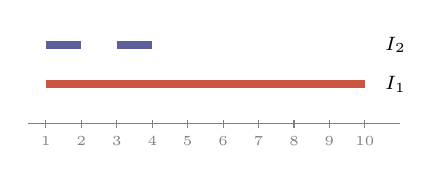
\begin{tikzpicture}[x=4.5mm,y=5mm, baseline=(base)]
\draw[gray] (0.5,0) -- (11,0); \foreach \xx in {1,...,10} {\draw[gray] (\xx,0.1) -- (\xx,-0.1); \node[font=\tiny, text=gray] at (\xx,-0.45) {\xx};}
\draw[line width=3pt, BrickRed!70] (1,1) -- (10,1); \node[font=\scriptsize, anchor=west] at (10.3,1) {$I_1$};
\draw[line width=3pt, MidnightBlue!70] (1,2) -- (2,2); \draw[line width=3pt, MidnightBlue!70] (3,2) -- (4,2); \node[font=\scriptsize, anchor=west] at (10.3,2) {$I_2$};
\coordinate (base) at (0,1);
\end{tikzpicture}
\hspace{1.5cm}
\begin{tikzpicture}[x=1.2cm,y=1cm, baseline=(base)]
\foreach \nm [count=\k] in {a,b,c,d} {\node[vtxs] (m\nm) at (\k,0.5) {$\nm$};}
\draw[line width=2.5pt, MidnightBlue!70] (ma) -- (mb); \draw[line width=2.5pt, BrickRed!70] (mb) -- (mc); \draw[line width=2.5pt, MidnightBlue!70] (mc) -- (md);
\coordinate (base) at (0,0.5);
\end{tikzpicture}
\end{figura}

\begin{complemento}[Para saber mais: interseção de matroides]
Dadas duas matroides $M_1=(E,\mathcal I_1)$ e $M_2=(E,\mathcal I_2)$, o problema da \textbf{interseção de matroides} pede um conjunto $I\in\mathcal I_1\cap\mathcal I_2$ de tamanho (ou peso) máximo. Vários problemas são desse tipo: o \emph{emparelhamento máximo em grafos bipartidos} é a interseção de duas matroides de partição (no máximo uma aresta por vértice de cada lado); a \emph{floresta colorida} --- o maior conjunto de arestas que é uma floresta e tem no máximo uma aresta de cada cor --- é a interseção da matroide gráfica com uma de partição pelas cores.

A interseção de duas matroides, em geral, não é uma matroide, e o guloso pode falhar, como no caminho $a\!-\!b\!-\!c\!-\!d$ acima, que é bipartido. Mesmo assim, o problema é \textbf{polinomial}, por um algoritmo de \emph{caminhos aumentantes}. Dado um conjunto comum $I$, constrói-se um \emph{grafo de troca}: para $y\in I$ e $x\notin I$, há um arco $y\to x$ se $I-y+x\in\mathcal I_1$ e um arco $x\to y$ se $I-y+x\in\mathcal I_2$; as fontes são os $x$ com $I+x\in\mathcal I_1$ e os destinos, os $x$ com $I+x\in\mathcal I_2$. Um caminho \emph{mais curto} de uma fonte a um destino dá, por diferença simétrica com $I$, um conjunto comum com um elemento a mais; se não há caminho, $I$ é máximo. São no máximo $r$ aumentos, cada um com $O(nr)$ consultas ao oráculo. Vale ainda um teorema de dualidade: $\max|I|=\min_{U\subseteq E}\{r_1(U)+r_2(E\setminus U)\}$.

Com \textbf{três} matroides, o problema já é NP-difícil: um \emph{caminho hamiltoniano} num digrafo é um conjunto comum de tamanho $n-1$ a três matroides --- a gráfica do grafo subjacente (sem ciclos), a de partição ``grau de entrada no máximo 1'' e a de partição ``grau de saída no máximo 1''. Também é polinomial o \textbf{particionamento} de matroides, que cobre $E$ com o menor número de independentes (por exemplo, cobrir as arestas de um grafo com o menor número de florestas). Reconhecer que um problema é uma interseção ou um particionamento de matroides prova, portanto, que ele é polinomial.
\end{complemento}

\begin{chave}
Guloso: escolha local, sem retrocesso; correto quando vale a propriedade gulosa, provada por troca. Matroide: (I1) $\emptyset$ independente, (I2) fechada para subconjuntos, (I3) aumento. Nas matroides, o guloso (ordem decrescente de peso e oráculo de independência) encontra a base de peso máximo, e apenas nelas ele acerta para todo peso. Exemplos: linear, gráfica, uniforme, de partição, transversal. Não exemplos: emparelhamentos de arestas e intervalos disjuntos. A interseção de duas matroides é polinomial; a de três, NP-difícil.
\end{chave}

% ----------------------------------------------------------------
\section{Exercícios}
\excurso
\begin{exercicio}{gm-troco}[Lista]
Escreva um algoritmo guloso para o problema do troco: dar $S$ centavos com o menor número de moedas, de valores $v_1,\dots,v_n$. Mostre que ele é ótimo para as moedas $\{10,5,2,1\}$ e que não é ótimo para qualquer sistema monetário.
\end{exercicio}
\begin{exercicio}{gm-i3}[Slides]
Prove o axioma de aumento (I3) para a matroide linear, para a gráfica, para a transversal e para a de emparelhamento.
\end{exercicio}
\begin{exercicio}{gm-g}[Slides]
Mostre que, se $\mathcal I$ satisfaz (I1) e (I2) e o algoritmo guloso devolve um independente maximal de peso máximo para \emph{toda} função de peso, então vale (I3).
\end{exercicio}
\begin{exercicio}{gm-pratica}[Slides]
(a) É possível usar matroides no problema de seleção de intervalos com pesos unitários? (b) Faça um algoritmo para verificar se um conjunto $S$ de vetores-coluna de uma matriz é linearmente independente. Qual a complexidade?
\end{exercicio}
\begin{exercicio}{gm-pesq}[Pesquisa]
Investigue: os axiomas das matroides e sua interpretação; a relação entre a propriedade de troca e a correção do guloso; o algoritmo de Kruskal como guloso numa matroide; quando a maximização de pesos pelo guloso é ótima; o que muda quando há duas famílias de restrições de independência; como funciona a interseção de duas matroides por caminhos aumentantes; e por que duas matroides levam a problemas polinomiais enquanto três já podem levar a problemas NP-difíceis.
\end{exercicio}

\excompl
\begin{exercicio}{gm-ativ}[Complementar]
Seleção de atividades: 11 atividades têm inícios $s=(1,3,0,5,3,5,6,8,8,2,12)$ e términos $f=(4,5,6,7,9,9,10,11,12,14,16)$. Aplique o guloso ``a que termina primeiro'' e prove que ele é ótimo.
\end{exercicio}
\begin{exercicio}{gm-ruins}[Complementar]
Mostre com contraexemplos que, para a seleção de atividades, os gulosos ``a de menor duração primeiro'' e ``a que começa primeiro'' não são ótimos.
\end{exercicio}
\begin{exercicio}{gm-frac}[Complementar]
Na mochila \emph{fracionária}, em que se podem levar frações dos itens, prove que o guloso pela razão valor/peso é ótimo. Aplique a $W=50$ e itens $(p,v)=(10,60),(20,100),(30,120)$ e compare com a mochila 0-1.
\end{exercicio}
\begin{exercicio}{gm-unif}[Complementar]
Prove que a matroide uniforme $U_{n,k}$ e a matroide de partição satisfazem (I1), (I2) e (I3).
\end{exercicio}
\begin{exercicio}{gm-tarefas}[Complementar \estrela]
Tarefas unitárias com prazos e multas: cada tarefa leva uma unidade de tempo, tem prazo $d_i$ e multa $w_i$ se terminar depois do prazo. Um conjunto de tarefas é \emph{independente} se pode ser executado todo dentro dos prazos, o que vale se e somente se, para todo $t$, no máximo $t$ tarefas do conjunto têm prazo $\le t$. Esses conjuntos formam uma matroide; use o guloso para minimizar a multa total com $d=(4,2,4,3,1,4,6)$ e $w=(70,60,50,40,30,20,10)$.
\end{exercicio}
\begin{exercicio}{gm-huffman}[Complementar \estrela]
Os \emph{códigos de Huffman} são construídos por um guloso que junta, repetidamente, as duas árvores de menor frequência. Construa o código para as frequências $a{:}45$, $b{:}13$, $c{:}12$, $d{:}16$, $e{:}9$ e $f{:}5$ e calcule o custo $\sum(\text{frequência})\times(\text{tamanho do código})$.
\end{exercicio}
\begin{exercicio}{gm-spt}[Complementar]
Tarefas com durações $t_1,\dots,t_n$ serão executadas uma após a outra numa única máquina. Mostre que executá-las em ordem crescente de duração minimiza a soma dos instantes de término. Aplique a durações $3,1,2$.
\end{exercicio}
\begin{exercicio}{gm-naomat}[Complementar]
Seja $E=\{1,2,3\}$ e $\mathcal I=\{\emptyset,\{1\},\{2\},\{3\},\{1,2\}\}$. Verifique se $(E,\mathcal I)$ é uma matroide. Em caso negativo, mostre uma função de peso para a qual o guloso falha.
\end{exercicio}
\begin{exercicio}{gm-paralelos}[Complementar]
Seja $E=\{1,2,3,4\}$ e $\mathcal I$ a família dos conjuntos com no máximo 2 elementos, exceto $\{1,2\}$. Verifique se é uma matroide e dê uma matriz cujas colunas realizam essa matroide.
\end{exercicio}
\begin{exercicio}{gm-posto}[Complementar]
Mostre que, na matroide gráfica de um grafo com $n$ vértices e $c$ componentes conexas, todas as bases têm $n-c$ arestas. Qual o posto da matroide gráfica de um grafo com 6 vértices formado por um triângulo e um caminho com 3 vértices?
\end{exercicio}
\begin{exercicio}{gm-dual}[Complementar]
Mostre que o dual da matroide uniforme $U_{n,k}$ é $U_{n,n-k}$.
\end{exercicio}
\begin{exercicio}{gm-unifgul}[Complementar]
O que faz o algoritmo guloso na matroide uniforme $U_{n,k}$? E numa matroide de partição? Aplique ao problema de escolher, entre itens das categorias $A=\{9,7,4\}$, $B=\{8,3\}$ e $C=\{6,5,2\}$ (os números são os pesos), no máximo 2 itens por categoria com peso total máximo.
\end{exercicio}
\begin{exercicio}{gm-moedas}[Complementar]
Mostre que o troco guloso não é ótimo para as moedas $\{1,7,10\}$, dando um valor $S$ em que ele falha. O sistema $\{1,5,10,25\}$ tem esse problema?
\end{exercicio}
\begin{exercicio}{gm-pesado}[Complementar]
Dê um exemplo de seleção de intervalos \emph{com pesos} em que o guloso ``o que termina primeiro'' não encontra o conjunto compatível de peso máximo. Como resolver esse problema?
\end{exercicio}
\begin{exercicio}{gm-fracn}[Complementar \estrela]
Mostre que a mochila fracionária pode ser resolvida em $O(n)$, sem ordenar os itens, usando seleção em tempo linear.
\end{exercicio}
